\chapter{A Simple Exact Algorithm}\label{ch:exact}
\section{The capped Delaunay dynamic program}\label{sec:dp}

Fix $r>0$ and write $\far$ for $\far_r$. For the decision problem it suffices
to consider \emph{chords} $(i,j)$ with $0\le i<j\le n-1$. A chord is
\emph{admissible} if $\far(i,j)$, and a point $p_l\in P(i,j)$ is an
\emph{admissible apex} of $(i,j)$ if $\far(i,l)$ and $\far(l,j)$. Let
\[
\Tr=\bigl|\{(i,l,j): 0\le i<l<j\le n-1,\ \far(i,l),\ \far(l,j),\ \far(i,j)\}\bigr|\le\tbinom n3
\]
be the number of $r$-far triples.

\begin{definition}\label{def:config}
Let $(i,j)$ be an admissible chord. An \emph{$(i,j)$-configuration} is a pair
$(X,T)$ where $X\subseteq P(i,j)$ and, if $X\neq\emptyset$, $T$ is a
triangulation of $X\cup\{p_i,p_j\}$ that satisfies (a) and (b) of
\cref{thm:cert-delaunay}. If $X\ne\emptyset$, the \emph{apex} of $(X,T)$ is
the third vertex $p_l$ of the triangle of $T$ containing the edge $p_ip_j$.
For $\varphi\in(0,\pi]$ let $F(i,j\mid\varphi)$ be the maximum of $|X|$ over
all $(i,j)$-configurations with $X=\emptyset$ or $\ang p_ip_lp_j\le\varphi$.
\end{definition}

The bound $\varphi$ encodes the triangle on the other side of the chord: if
$p_ip_j$ is a diagonal of a larger triangulation whose other triangle at
$p_ip_j$ is $p_ip_jp_t$, then by~\eqref{eq:ld} the diagonal is locally
Delaunay exactly if $\ang p_ip_lp_j\le\pi-\ang p_ip_tp_j$. See
\cref{fig:dp}.

\begin{figure}[tb]
\centering
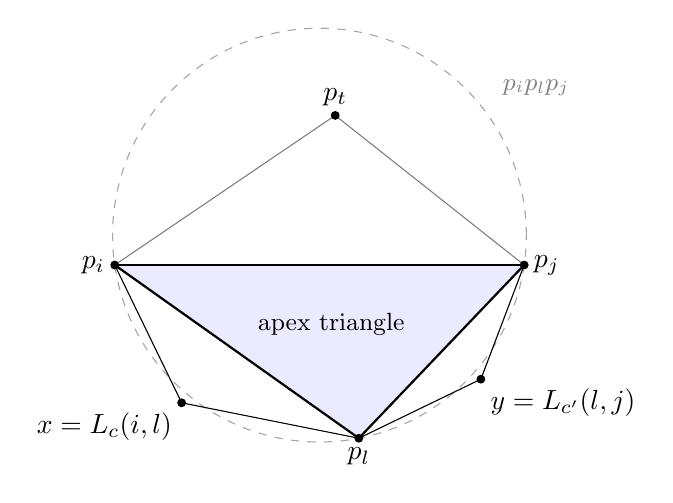
\begin{tikzpicture}[scale=1.0,>=stealth]
  \coordinate (i) at (-2.6,0);
  \coordinate (j) at (2.6,0);
  \coordinate (l) at (0.5,-2.2);
  \coordinate (x) at (-1.75,-1.75);
  \coordinate (y) at (2.05,-1.45);
  \coordinate (t) at (0.2,1.9);
  % circle through i, l, j: centre (0, c) with c = (0.25+4.84-6.76)/(-4.4)
  \draw[gray!70,dashed] (0,0.3795) circle (2.6276);
  \fill[blue!8] (i)--(l)--(j)--cycle;
  \draw[thick] (i)--(j);
  \draw[thick] (i)--(l)--(j);
  \draw (i)--(x)--(l);
  \draw (l)--(y)--(j);
  \draw[gray] (i)--(t)--(j);
  \foreach \p/\pos/\lab in {i/left/{$p_i$}, j/right/{$p_j$}, l/below/{$p_l$}, x/below left/{$x=L_c(i,l)$}, y/below right/{$y=L_{c'}(l,j)$}, t/above/{$p_t$}}
    {\fill (\p) circle (1.6pt); \node[\pos] at (\p) {\lab};}
  \node at (0.15,-0.75) {\small apex triangle};
  \node[gray] at (2.75,2.25) {\small $\circlethree{p_i}{p_l}{p_j}$};
\end{tikzpicture}
\caption{A chord $(i,j)$ with apex $p_l$. The sub-configuration of $(i,l)$
with apex $x$ is compatible with the triangle $p_ip_lp_j$ iff $x$ is not
strictly inside $\circlethree{p_i}{p_l}{p_j}$ (here: $x$ is outside); likewise
for $y$ and $(l,j)$. The parent triangle $p_ip_jp_t$ constrains $p_l$ in the
same way.}
\label{fig:dp}
\end{figure}

\begin{lemma}[Recurrence]\label{lem:rec}
For every admissible chord $(i,j)$ and every $\varphi\in(0,\pi]$,
\[
F(i,j\mid\varphi)=\max\Bigl(\{0\}\cup\bigl\{\,v(l) : p_l\text{ admissible apex of }(i,j),\ \ang p_ip_lp_j\le\varphi\bigr\}\Bigr),
\]
where
$v(l)=1+F\bigl(i,l\mid\pi-\ang p_ip_jp_l\bigr)+F\bigl(l,j\mid\pi-\ang p_lp_ip_j\bigr)$.
\end{lemma}
\begin{proof}
($\ge$) Let $p_l$ be an admissible apex with $\ang p_ip_lp_j\le\varphi$, and
let $(X_1,T_1)$ and $(X_2,T_2)$ be optimal configurations of $(i,l)$ and
$(l,j)$ under the bounds in the definition of $v(l)$. Put
$X=X_1\cup X_2\cup\{p_l\}$ and let $T$ consist of $T_1$, $T_2$ and the
triangle $p_ip_lp_j$. The three sides of this triangle have length at least
$r$. If $X_1\ne\emptyset$, then $p_ip_l$ is a diagonal of $T$ whose two
triangles are $p_ip_lp_j$ and the apex triangle of $T_1$, and
by~\eqref{eq:ld} the bound $\pi-\ang p_ip_jp_l$ on the apex angle of $T_1$ is
exactly its local Delaunay condition; symmetrically for $p_lp_j$. All other
diagonals of $T$ are diagonals of $T_1$ or $T_2$. So $(X,T)$ is an
$(i,j)$-configuration with apex $p_l$ and $|X|=v(l)$.

($\le$) Let $(X,T)$ be an optimal configuration with $X\ne\emptyset$ and apex
$p_l$. By (a), $p_l$ is an admissible apex. Removing the triangle $p_ip_lp_j$
splits $T$ into triangulations of $(X\cap P(i,l))\cup\{p_i,p_l\}$ and
$(X\cap P(l,j))\cup\{p_l,p_j\}$, which are configurations of $(i,l)$ and
$(l,j)$, and by (b) their apex angles obey the bounds in $v(l)$. Hence
$|X|\le v(l)$.
\end{proof}

\begin{theorem}[Decision]\label{thm:decision}
Let $k\ge3$. $P$ has an $r$-far $k$-set if and only if some admissible chord
$(i,j)$ has $F(i,j\mid\pi)\ge k-2$.
\end{theorem}
\begin{proof}
($\Rightarrow$) Let $S$ be an $r$-far $k$-set, let $p_i$ and $p_j$ be its
points of smallest and largest index, and let $T$ be a Delaunay triangulation
of $S$. Then $X=S\setminus\{p_i,p_j\}\subseteq P(i,j)$ and $(X,T)$ is an
$(i,j)$-configuration by \cref{thm:cert-delaunay}, with $|X|=k-2$.
($\Leftarrow$) A configuration $(X,T)$ with $|X|\ge k-2\ge 1$ is a
triangulation of $X\cup\{p_i,p_j\}$ satisfying (a) and (b). By
\cref{thm:cert-delaunay} this set is $r$-far, and any $k$ of its points form
an $r$-far $k$-set.
\end{proof}

\subsection{Thresholds: \texorpdfstring{$k-2$}{k-2} apex points per chord}

Evaluating the recurrence naively needs one table entry per chord and apex and
$O(n)$ work per entry, that is, $O(n^4)$ time. The following observation
removes a factor~$n$ and, with capping, replaces $\log n$ by $\log k$.

Fix an admissible chord $(i,j)$. For $c\ge1$ define the \emph{$c$-th
threshold}
\[
\tau_c(i,j)=\min\bigl\{\ang p_ip_lp_j : p_l\text{ admissible apex of }(i,j),\ v(l)\ge c\bigr\},
\]
with $\tau_c(i,j)=+\infty$ if no such apex exists, and put $\tau_0=0$.

\begin{lemma}\label{lem:thresholds}
For every admissible chord, $\tau_1\le\tau_2\le\cdots$ and
$F(i,j\mid\varphi)=\max\{c\ge0:\tau_c(i,j)\le\varphi\}$. Moreover, for every
integer $K\ge1$, the thresholds $\tau_1,\dots,\tau_K$ of a chord are determined
by the thresholds $\tau_1,\dots,\tau_K$ of shorter chords.
\end{lemma}
\begin{proof}
The sets $\{l:v(l)\ge c\}$ shrink as $c$ grows, which gives monotonicity. By
\cref{lem:rec}, $F(i,j\mid\varphi)\ge c$ iff some admissible apex $p_l$ with
$\ang p_ip_lp_j\le\varphi$ has $v(l)\ge c$, iff $\tau_c\le\varphi$. For the
last claim write $F_K=\min(F,K)$. The thresholds $\tau_1,\dots,\tau_K$ depend
on $v$ only through $\min(K,v)$, and
$\min(K,v(l))=\min\bigl(K,1+F_K(i,l\mid\cdot)+F_K(l,j\mid\cdot)\bigr)$, where
$F_K$ of a chord is determined by its first $K$ thresholds.
\end{proof}

For a dispersion query we only need to know whether $F\ge k-2$, so we set
$K=k-2$ and keep $K$ thresholds per chord. We do not store angles: we store
$\tau_c(i,j)$ as an apex $L_c(i,j)$ that attains it ($L_c=\nil$ if
$\tau_c=+\infty$). Then, for an admissible apex $p_l$ of $(i,j)$ and
$x=L_c(i,l)$,
\[
F_K\bigl(i,l\mid\pi-\ang p_ip_jp_l\bigr)\ge c
\iff \ang p_ixp_l+\ang p_ip_jp_l\le\pi
\iff x\text{ is not strictly inside }\circlethree{p_i}{p_l}{p_j}
\]
by (I2), since $x$ and $p_j$ lie on opposite sides of the line $p_ip_l$. The
same circle answers the query for the chord $(l,j)$. Each query is monotone in
$c$, so the number of thresholds that pass is found by binary search with
$O(\log K)$ in-circle tests. Comparing the apex angles of two apexes $p_l$,
$p_{l'}$ of the same chord is the in-circle test~(I1). \Cref{alg:capped}
gives the complete procedure.

\begin{algorithm}
\caption{$\AlgCapped(P,k,r)$\quad ($k\ge3$, $K=k-2$)}\label{alg:capped}
\begin{tabbing}
\hspace{1.4em}\=\hspace{1.4em}\=\hspace{1.4em}\=\hspace{1.4em}\=\kill
\textbf{for} $g=2,\dots,n-1$ \textbf{do}\` \emph{chords by increasing length $j-i$}\\
\>\textbf{for each} admissible chord $(i,j)$ with $j=i+g$ \textbf{do}\\
\>\>$best[1..K]\gets\nil$\\
\>\>\textbf{for each} admissible apex $p_l$ of $(i,j)$ \textbf{do}\` \emph{bit-parallel enumeration}\\
\>\>\>$q_1\gets\#\{c: L_c(i,l)\ne\nil\text{ is not strictly inside }\circlethree{p_i}{p_l}{p_j}\}$\` \emph{binary search}\\
\>\>\>$q_2\gets\#\{c: L_c(l,j)\ne\nil\text{ is not strictly inside }\circlethree{p_i}{p_l}{p_j}\}$\` \emph{binary search}\\
\>\>\>$v\gets\min(K,1+q_1+q_2)$\\
\>\>\>\textbf{if} $best[v]=\nil$ or $\ang p_ip_lp_j<\ang p_i\,best[v]\,p_j$ \textbf{then} $best[v]\gets p_l$\\
\>\>\textbf{for} $c=K,\dots,1$ \textbf{do} $L_c(i,j)\gets$ apex of smallest angle among $best[c..K]$\` \emph{suffix minima}\\
\>\>\textbf{if} $L_K(i,j)\ne\nil$ \textbf{then return} \textsc{true}\\
\textbf{return} \textsc{false}
\end{tabbing}
\end{algorithm}

\begin{theorem}\label{thm:decision-alg}
\Cref{alg:capped} decides whether $P$ has an $r$-far $k$-set in
\[
O\bigl(n^2k+n^3/w+\Tr\log k\bigr)\ \subseteq\ O(n^3\log k)
\]
time and $O(n^2k)$ space. If the answer is positive, an $r$-far $k$-set can be
reported in $O(k\log k)$ additional time.
\end{theorem}
\begin{proof}
\emph{Correctness.} By induction on $j-i$, after the chord $(i,j)$ has been
processed, $L_c(i,j)$ attains $\tau_c(i,j)$ for $1\le c\le K$: the counts
$q_1,q_2$ equal $F_K$ of the two sub-chords under the bounds of
\cref{lem:rec} by the discussion above, so $v=\min(K,v(l))$; $best[v]$ is an
apex of smallest angle among the apexes with capped value exactly $v$, and the
suffix minima give the apexes of smallest angle with capped value at least
$c$. By \cref{lem:thresholds} and \cref{thm:decision}, an $r$-far $k$-set
exists iff $\tau_K(i,j)\le\pi$, i.e.\ $L_K(i,j)\ne\nil$, for some chord.

\emph{Running time.} Initialising and finishing a chord costs $O(K)$. The
admissible apexes of $(i,j)$ are the positions $l\in(i,j)$ where the rows of
$p_i$ and $p_j$ in the bit matrix of the relation $\far$ both have a one; they
are enumerated in $O(n/w)$ time plus $O(1)$ per apex. The body of the inner
loop is executed once per $r$-far triple and costs $O(\log K)$.

\emph{Witness.} Starting from a chord with $L_K\ne\nil$ and demand $c=K$,
take $p_l=L_c(i,j)$, recompute $q_1$ for $p_l$, and recurse on $(i,l)$ with
demand $c_1=\min(q_1,c-1)$ and on $(l,j)$ with demand $c-1-c_1\le q_2$. The
recursion visits at most $K$ chords and performs one binary search in each.
The reported points together with $p_i,p_j$ form the vertex set of a
configuration and are $r$-far by \cref{thm:cert-delaunay}.
\end{proof}

\begin{remark}[The role of the cap]\label{rem:cap}
With $K=n-2$ nothing is truncated and $2+\max_{(i,j)}F(i,j\mid\pi)$ is the
maximum size of an $r$-far subset, in $O(n^3\log n)$ time and $O(n^3)$ space;
this matches the bound of~\citet{tw26} in the unweighted unit case. Capping
reduces the logarithm to $\log k$, the space to $O(n^2k)$, and allows the
early exit in the last line of the loop. The $\log k$ factor is only paid on
$r$-far triples; in the upper part of the search window many triples are not
$r$-far.
\end{remark}

\paragraph{Maximum independent sets.}
The cap can also be chosen adaptively. Let $\alpha=\alpha_r(P)$ be the maximum
size of an $r$-far subset of $P$, i.e.\ the independence number of the graph on
$P$ in which two points are adjacent iff their distance is smaller than $r$
(the unit-disk graph, after scaling).

\begin{corollary}\label{cor:mis}
A maximum $r$-far subset of $n$ points in convex position can be computed in
$O(n^2\alpha+n^3/w+\Tr\log\alpha)\subseteq O(n^3\log\alpha)$ time and
$O(n^2\alpha)$ space, where $\alpha$ is its size.
\end{corollary}
\begin{proof}
Compute an inclusion-maximal $r$-far set $M$ greedily in $O(n|M|)$ time. Every
point of $P$ is at distance less than $r$ from some point of $M$, and an open
disk of radius $r$ contains at most five points of any $r$-far set (among six
points other than the centre, two would subtend an angle of at most $\pi/3$ at
the centre and would therefore be closer than $r$; and if the centre belongs
to the set, no other point of the disk does).
Hence $|M|\le\alpha\le5|M|$. Run \cref{alg:capped} with
$K=\min(n,5|M|)-1$ and without the early exit. Since $F\le\alpha-2<K$, no
value is truncated, so the maximum number of finite thresholds over all chords
equals $\alpha-2$ if $\alpha\ge3$, and a witness is reconstructed as in
\cref{thm:decision-alg}. If there is no $r$-far triple, the answer is an
$r$-far pair or a single point.
\end{proof}

\section{Optimisation and the search window}\label{sec:opt}

The optimum $\rstar$ is one of the $\binom n2$ pairwise distances, and
feasibility is monotone in $r$, so $\rstar$ can be found by binary search over
the sorted distinct distances with \cref{alg:capped} as the oracle. The
following window shrinks the search range before any exact decision is made.

\begin{lemma}[Search window]\label{lem:window}
Let $G$ be a farthest-first $k$-set of $P$ (start with an arbitrary point and
repeatedly add a point whose distance to the chosen points is largest), and
let $g=\delta(G)$. Then for $k\ge3$
\[
g\ \le\ \rstar\ \le\ \min\bigl\{2g,\ \per(P)/k\bigr\}.
\]
\end{lemma}
\begin{proof}
$g\le\rstar$ because $G$ is a feasible $k$-set. Let $G'$ be the set of the
first $k-1$ points chosen. The distances at which points are added are
non-increasing, so $g$ is the distance from the last point to $G'$, and every
point of $P$ is within distance $g$ of $G'$ (this is Gonzalez's
argument~\citep{gonzalez}). Two of the $k$ points of an optimal set have the
same nearest point in $G'$, hence $\rstar\le2g$. Finally, let $S^*$ be an
optimal set. Then $\conv(S^*)$ is a convex $k$-gon whose sides have length at
least $\rstar$, so its perimeter is at least $k\rstar$; since
$\conv(S^*)\subseteq\conv(P)$ and the perimeter of convex sets is monotone
under inclusion, $k\rstar\le\per(P)$.
\end{proof}

\begin{theorem}\label{thm:opt}
The $k$-dispersion problem for $n$ points in convex position can be solved in
$O(n^3\log k\log n)$ time and $O(n^2k)$ space. More precisely, the time is
$O(n^2\log n)$ plus $O(\log n)$ calls to \cref{alg:capped}.
\end{theorem}
\begin{proof}
For $k=2$ the answer is the diameter. For $k\ge3$, sort the distinct pairwise
distances, restrict them to the window of \cref{lem:window} (computing $G$
takes $O(nk)$ time), and binary search with \cref{alg:capped}; the value $g$
is known to be feasible. The witness of the last positive call, or $G$ if there
is none, is an optimal set.
\end{proof}

\subsection{A certified algorithm}\label{sec:certified}

Although no seeded rule is complete, all of them are \emph{sound}: they only
ever output $r$-far sets. So a successful greedy run at radius $\rho$ proves
$\rstar\ge\rho$, and a single exact decision just above $\rho$ can prove
$\rstar\le\rho$. \Cref{alg:certified} combines the two. As heuristic predicate
$H(r)$ we use the alternating greedy from all seeds $\{q,a(q)\}$ and
$\{q,a(q),b(q)\}$ with both starting sides.

\begin{algorithm}[H]
\caption{$\AlgCert(P,k)$\quad ($k\ge3$)}\label{alg:certified}
\begin{enumerate}[label=\arabic*:,leftmargin=2em,itemsep=1pt,topsep=2pt]
\item $W\gets$ the sorted distinct distances inside the window of \cref{lem:window};\ \ $\rho\gets g$, which is feasible.
\item Binary search on $W$ with the predicate $H$; let $\rho$ be the largest radius at which a run succeeded.
\item Let $\rho^+$ be the successor of $\rho$ in $W$. \textbf{If} $\rho=\max W$ \textbf{or} $\AlgCapped(P,k,\rho^+)$ is \textsc{false}, \textbf{return} $\rho$.
\item Otherwise $\rho^+$ is feasible: \textbf{return} the result of binary search on $W\cap[\rho^+,\infty)$ with $\AlgCapped$.
\end{enumerate}
\end{algorithm}

\begin{theorem}\label{thm:cert}
\Cref{alg:certified} returns $\rstar$ on every input. It runs in
$O(n^2k\log n+n^3\log k)$ time whenever $\rho=\rstar$ after the heuristic
phase, and in $O(n^3\log k\log n)$ time in the worst case.
\end{theorem}
\begin{proof}
Every success of $H$ exhibits an $r$-far $k$-set and $g$ is feasible, so
$\rho\le\rstar$ regardless of whether $H$ is monotone. If $\rho=\max W$, then
$\rho=\rstar$ by \cref{lem:window}. If the exact decision at $\rho^+$ fails,
then $\rstar<\rho^+$ and hence $\rstar=\rho$, because $\rstar\in W$. Otherwise
$\rstar\ge\rho^+$ and the exact binary search finds it.

For the running time, $a(q)$ and $b(q)$ are found for all $q$ in $O(n^2)$
time. In one greedy run each frontier only moves forward, and a point that is
skipped is never examined again from that side, so a run examines $O(n)$
points and compares each with at most $k$ chosen points. There are $4n$ runs
per evaluation of $H$ and $O(\log n)$ evaluations, followed by a single call
to \cref{alg:capped} if $\rho=\rstar$.
\end{proof}

